\documentclass[main.tex]{subfiles}
%\bibliography{bibilo}
\begin{document}
\graphicspath{{img/}{../img/}}

%% TODO %%


% cite book I used 
% define utils.py methods
% define managers.py methods

\section{Methodology}
The following section outlines the various components of tracker and how they are connected and controlled programmatically. 
\subsection{Tracker Overview}
The components of the tracker are as follows:
\begin{itemize}
\item \textit{base}
  \begin{itemize}
  \item 2 stepper motors
  \item EiBotBoard (motor controller)
  \item X-Y translation mechanism 
  \item camera
  \end{itemize}

\item \textit{housing}
  \begin{itemize}
  \item elevation rig
  \item dish stage
  \item lighting mount
  \item lighting diffuser
  \end{itemize}

\item \textit{computer}
\end{itemize}


The \textit{base} and \textit{housing} components (see Figure \ref{fig:rig}) are modular, meaning any housing can be used with any base. This also allows for easy transport. \\

\begin{figure}[!htbp]
  \centering
  \includegraphics[scale = 0.08]{zoom-in-rig}
  \caption{\textit{housing} and \textit{base}}
  \label{fig:rig}
\end{figure}


The \textit{base} (see Figure \ref{fig:x-y}) module houses the hardware of the system. The \textit{camera} is mounted on the \textit{X-Y translation mechanism}, whose movement is controlled by two \textit{stepper motors} connected to an \textit{EiBotBoard (EBB)}.The \textit{housing} module elevates the \textit{dish stage} above the camera. 

\begin{figure}[!htbp]
\centering
\includegraphics[scale=0.08]{x-y2}
\caption{Close-up of \textit{base}}
\label{fig:x-y}
\end{figure}




It is important to note that the \textit{dish stage} (see Figure~\ref{fig:dish})  needs to be co-planar with the \textit{base} for a flat field (to maintain focus of the camera on all areas of the dish). This component can also be raised or lowered to allow for different field resolutions, allowing to worms take up more or less frame space (ie. zoom). \\ %better word?
\begin{figure}[!htbp]
  \centering
  \includegraphics[scale = 0.08]{dish}
  \caption{15cm \textit{dish} on \textit{dish stage}}
  \label{fig:dish}
\end{figure}



\subsection{Hardware}
This section specifies hardware parts used, pricing, and references to purchasing websites.
\subsubsection{Motors and Motor Control Board}
The stepper motors being used are easily available from the Evil Mad Scientist website~\cite{EvilMadmotor}. The price point is \$ 16/motor.\\

The motor control board is the \verb|EggBotBoard| \cite{EvilMadEBB}. The price point is \$50. 

\subsubsection{Imaging}
The current camera being used is e-con System's \verb|See3CAM_10CUG|. \cite{EconCam} It is a 1.5MP USB 3.0 camera capable of up to 45 fps at a resolution of 1280 $\times$ 960. It is a monochrome camera capable of delivering directly in FOURCC code GREY format. It can also deliver images in YUYV format. It is important to note that other cameras may be compatible with the system.

\subsubsection{Computer}
We are using a computer dedicated to the tracking system, though any laptop with similar configuration (outlined in Appendix~\ref{app:install}) should be compatible. The computer is the Intel NUC DN2820FYKH \cite{NUC} with 8GB RAM, 500GB HD, and 2.4GHz dual-core Celeron cpu. It's quite small (4" x 4" x 2"). Most importantly, it has a USB 3.0 for the camera. The price point is \$300.\\

\subsection{Software}
The tracking sofware was developed using the OpenCV 3.0.0 (dev) library \cite{OpenCV} in Python. The implementation leverages the fact OpenCV's Python library is bound to methods written in C++ and handles memory allocation, and interfaces with the \verb|video4linux (V4L & V4L2)| camera drivers (for devices called ``UVC compatible''). \\

This section specifies the algorithms and methods used specifically for finding the location of the worm in an image and deciding when to re-center the worm in the field of view. Also, it provides specification on how the images are captured from the camera and how the worm location is dispatched to the motor control board to move the camera.

\subsubsection{Finding the Worm}
The algorithm implemented for finding the worm is based on a simple motion tracking mechanism: the difference image. It leverages the fact that immobile background artifacts (like tracks or dips) subtract out to black, leaving only the moving worm as a white object in the difference image. The maximum pixel intensity in the difference image appears to always locate the worm, though no guarantee is placed that this point is the same on the worm's body frame to frame, or that it coincides with the centroid (center of mass). \\


\begin{algorithm}[h]
    \KwData{current frame, reference frame}
    \KwResult{wormLocation (row,col)}
    \While{frame from camera}
    {
        \eIf{have reference frame and camera not just moved}
        {
            subtracted image = reference frame - current frame\;
            \If{confidence in cropping}
            {
                crop subtracted image\;
            }
            {        
                blur subtracted image\;
                get maximum pixel intensity in blurred subtracted image\;
                update wormLocation\;
                set justMoved to False\;
            }   
    }{
    set current image as reference image\;}
}
\caption{findWorm}
\end{algorithm}

The \verb|findWorm()| method is only called at a rate of 10 fps, subsampling from the stream being emitted by the camera. This ensures more guarantees that the worm will not subtract itself out. To further improve the localization of the worm, a Gaussian smoothing filter ($\sigma = 9, n = 45 \times 45$) is also applied.\\ 

For efficiency when applying the Gaussian smoothing function, the space in the image in which the worm is sought is restricted by cropping (\verb|calculateCrop()|) during times when the confidence is high that the worm still resides in the \verb|cropRegion| of the frame being processed. The \verb|cropRegion| is always centered on the previous sample's \verb|wormLocation|. The cropping mechanism is in action after variable \verb|nPauseFrames| (current 20 frames) have elapsed, following the program start-up and after the camera has moved.\\

Necessarily, a new reference image is acquired after the camera has moved and is done in the \verb|decideMove()| method (specified in~\ref{ss:center}). \\

In the code, this method is called the \verb|processFrame()| method as part of the \verb|Finder| class in the \verb|finder.py| module. 

\clearpage
\subsubsection{Deciding When to Re-center the Worm in the Field of View}
\label{ss:center}
The algorithm for the \verb|move()| decision engine, was built trying to minimize heuristics for generalization to worms of any speed or activity. \\

\begin{algorithm}[h]
    \KwData{wormLocation (row, col)}
    \KwResult{Move or not move motors}
    \If{not on break and has reference image}
    {
        \If{reference image is old}
        {
            get new reference image\;
        }
        \If{wormLocation is outside boundary}
        {
            \If{wormLocation is not ridiculous}
            {
                set justMoved to True\;
                clear reference image\;
                start break\;
                center the worm\;
            }
        }
    }
\caption{decideMove}
\end{algorithm}
The current length of time during which the motors will be on break after a move has just been completed, is set to 3 sec (by \verb|breakDuration|). This ensures that the motors won't continually move. It corrects for possible localization errors after the camera has moved and a new reference image is being used. This is a very important check. It's possible that the \verb|justMoved| flag is redundant. \\

A frame reference is considered old if is has been used for more than \verb|REFPING| seconds (currently set to 600,000, and hence never called). This method was included for worms who are almost immobile or remain in a certain area. When the reference frame is old, subtracting the current and reference frames removes the worm, which then receives no location. Its utility has not been tested since the Gaussian blur was added to the \verb|findWorm| implementation. \\

A worm location is considered to be outside the boundary if it is outside the rectangle formed by \verb|boundRows|, \verb|boundCols| centered about the center of the frame. \\

A worm location is considered ridiculous if it is above a threshold set in \verb|MAXONEFRAME| (currently set to 500 pixels). Anecdotally, this filtering mechanism has not evaluated to True since a Gaussian blur was added to the \verb|findWorm()| method, and may not be necessary.\\ 

It is important to note that the parameters \verb|boundCols, boundRows|, \verb|MAXONEFRAME| and \verb|REFPING| are set in the \verb|finderArgs| dictionary in the \verb|Tracker| class defined in the \verb|tracking.py| module. This was mostly done to set many of the parameters that were changed often during testing to one place. These parameters are passed as arguments to the \verb|Finder| object when initialized from \verb|Tracker| object. 



The underlying geometry of these constructs in illustrated in Figure~\ref{fig:geom}

\begin{figure}[!htbp]
  \centering
  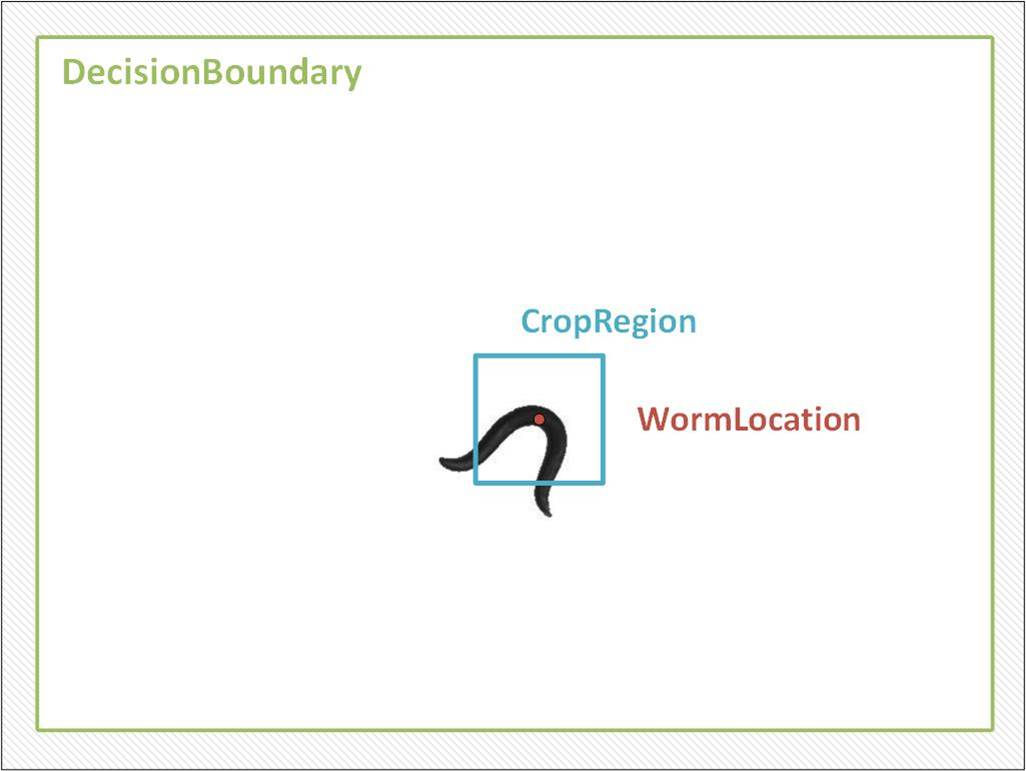
\includegraphics[scale = 0.5]{geom}
  \caption{Geometry of the \texttt{findWorm} and \texttt{decideMove()} methods}
  \label{fig:geom}
\end{figure}

The schematic, detailed overview of the system can be seen in Figure~\ref{fig:system}. 

\begin{figure}[!htbp]
  \centering
  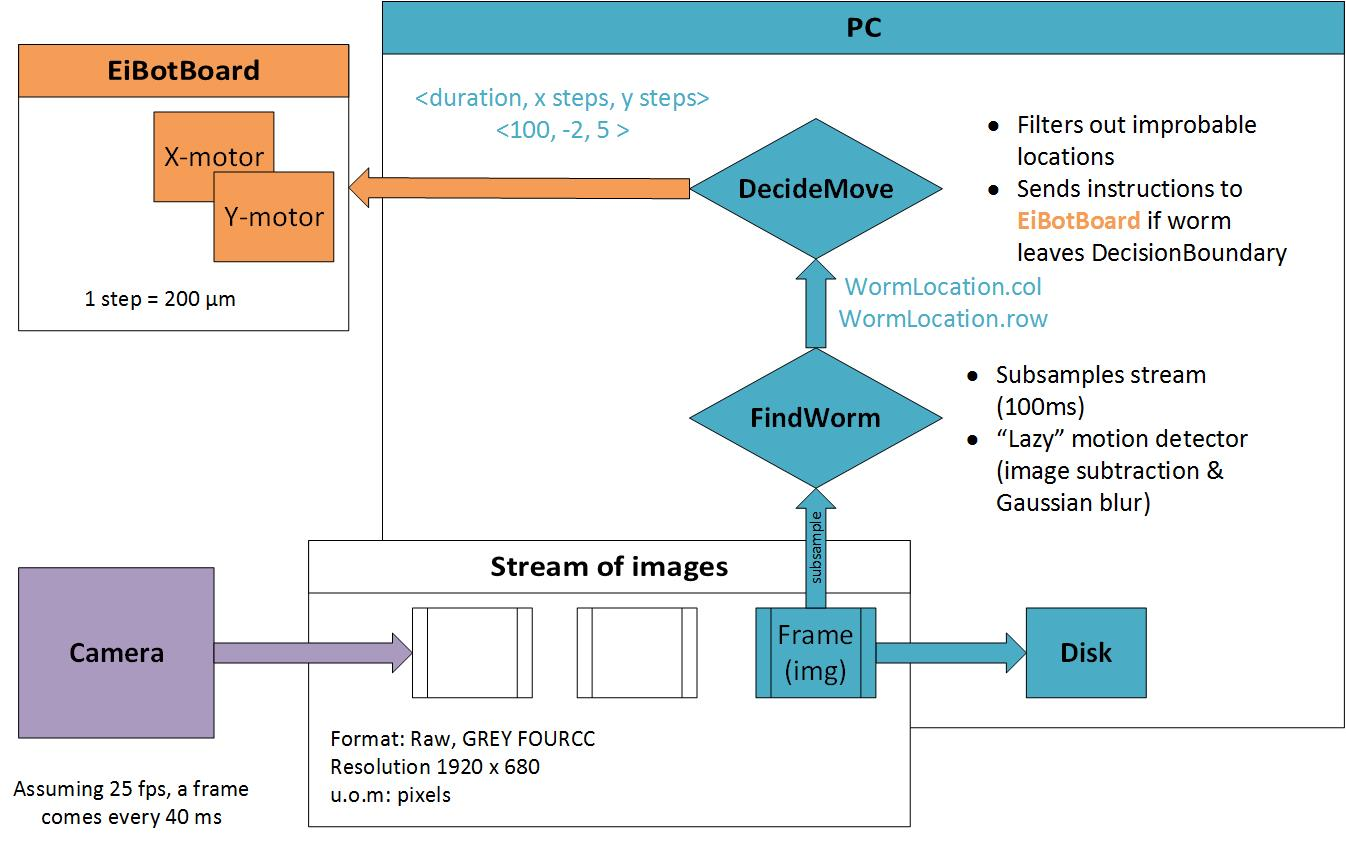
\includegraphics[scale = 0.5]{system}
  \caption{System diagram}
  \label{fig:system}
\end{figure}



\subsubsection{Linking Hardware to Software}
\label{sss:hslink}
\paragraph{Motors}
One of the main motivations to use python to write this software is that there exists sample code for sending instructions to the EBB. \cite{EBBsite, EBBcode}. The module \verb|easyEBB.py| defines the \verb|easyEBB| class and all methods related to motor control. A brief selection is outlined below:
\begin{itemize}
\item \verb| __init__(resolution, sizeMM, stepMode)| instantiates an \verb|easyEBB| object with the following parameters (and associated defaults):
  \begin{itemize}
  \item \verb|resolution = (1280,960)|
    \item \verb|sizeMM = 10| (the default frame width in mm)
    \item \verb|stepMode = 5| (full step mode)
  \end{itemize}
\item \verb|centerWorm( self, duration, colWormPix, rowWormPix )|: besides constructor (and destructor), is the only method called from the client code. Given a worm at pixel location \verb|(rowWormPix ,colWormPix)|, it will convert the pixel instructions (to center worm) to motor step instructions (\verb|move| method). It is important to note that the motors will only move in integer step instructions, meaning the camera may not move exactly to the desired location.

[Note: it has been requested by collaborator Dr. Christopher Brandon to send the move commands separately for X and Y directions to limit vibration]  
\item \verb|pixUmStepConversions( self, stepMode )|: uses resolution and frame width (in mm) to convert pixel measurements to steps. 
\item \verb|move( self, duration, xstep, ystep )|: sends move command to motor control board

\item Driver methods:
  \begin{itemize}
  \item \verb|openSerial()|: scans the \verb|\dev| folder for EBB and opens serial connection
  \item \verb|closeSerial()|: closes the serial connection opened above
  \item \verb|enableMotors()|: when serial connection is open, enables motors to receive \verb|move| commands
  \item \verb|disableMotors()|: when serial connection is open, disables motors from receiving \verb|move| commands
  \end{itemize}
\end{itemize}

 The motors can operate at full step (200 $\mu$m/step) or in fractional steps (e.g.: $1/2, 1/4, ...$). It is preferred to use full steps due to its precision over the fractional step modes. It is possible to instantiate the EBB object \verb|easyEBB| in fractional mode in the constructor by assigning the keys from the \verb|stepOpts| dictionary to the \verb|stepMode| variable:
\begin{verbatim}
        self.stepOpts = {1: 1./16, 
                         2: 1./8, 
                         3: 1./4, 
                         4: 1./2, 
                         5: 1}
\end{verbatim}




\paragraph{Acquiring images from the camera}
\label{p:Camera}
Despite this camera being touted as UVC compatible, many of the traditional UVC driver queries are not behaving nicely with the OpenCV driver interface. This includes querying frame rate.\\

In order to get our camera to read in images with the OpenCV library, changes need to be made in the OpenCV library source file: \verb|opencv\modules\highgui\bin\cap_libv4l.cpp|. The lines to change and how to change them are outlined in Table~\ref{table:srcChange} in Section~\ref{app:change}. These changes currently make the system only compatible with grayscale cameras. The underlying issue here is that the conversion of BGR24 to GREY was assumed possible for every camera by the OpenCV authors, but it did not seem to be the case for our system. The developers of the camera in India make claim that they were able to use the OpenCV library with no issues but their resolution was never able to be replicated.\\

Generally, however, the OpenCV implementation of capturing images from a camera is illustrated below. \\
\begin{lstlisting} 
#instantiation
cap = CaptureManager( 
         cv2.VideoCapture(captureSource), 
         window, 
         mirroredPreview, 
         resolution)
#use
while window.isWindowCreated:
    cap.grab()
    frame = cap.retrieve()
    window.show(frame)
\end{lstlisting}

\paragraph{Writing images to video}
The video is written leveraging OpenCV's \verb|VideoWriter| object. When writing frames, the  FOURCC MJPG codec writes in color format (which is a little unfortunate) using a frame rate estimate calculated after each frame is 'exited'. This estimate, however, changes over time. Troubling, is the fact that the VideoWriter gets instantiated only once with a frame rate estimate at that time, which unfortunately is variable over the length of capture. A small example of instantiation of the \verb|VideoWriter| object and the line used to write a frame is shown below. \\

\begin{lstlisting}
#instantiation
videoWriter = cv2.VideoWriter( videoFilename, 
                               videoEncoding, 
                               fps, 
                               size, 
                               color = False )
#use
videoWriter.write(frame)
\end{lstlisting}

\paragraph{Calibration}
Depending on the distance between the camera and the petri dish, the field of view will change. The calibration procedure involves initializing the \verb|easyEBB| object with the width of the frame in mm. There is a command line flag specified during launch of the tracker (\verb|-m conf|) that will draw two dots on the image coming from the camera. One is at pixel location (200, 300) and the other is in the center of the frame. To verify the measurement, a microscopic target should be positioned at the (200, 300) dot and the script \verb|dotTest.py| is run. If the target lands in at the center dot, then calibration is complete. If not, a more accurate measurement of the width of the frame should be attempted. 


\subsubsection{Main Thread}
The main thread connecting the video capture, processing, and recording methods is declared the \verb|tracker.py| file as \verb|run()| and was inspired from a project described in \cite{OpenCVPython}. It controls and redirects the program flow depending on parameters such as the presence of motors or the color format of the input image stream (to toggle video and camera sources). To start recording, the TAB key is pressed once and then again to stop recording. The ESC key exits the program entirely (with safe guards to end recording and close the serial connection to the motors). A minimalist GUI is provided by OpenCV which displays images using the \verb|show()| method. This allows display of an overlayed image in which \verb|wormLocation| can be drawn and verified by a human watching the video. 
\end{document}